\chapter{程式講解}
\section{變色程式講解}
\begin{figure}[hbt!]
\begin{center}
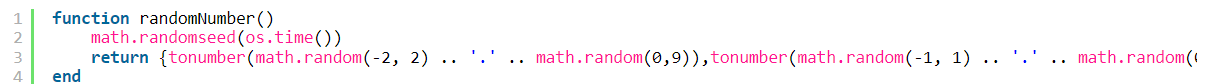
\includegraphics[width=12cm]{1}
\caption{\Large 改變顏色程式1}\label{改變顏色程式1}
\end{center}
\end{figure} 
這段程式碼,如(圖.\ref{改變顏色程式1}),定義了一個名為randomNumber的函數,當被呼叫時,它會產生一個由三個數字組成的列表list,這三個數字是從指定範圍中隨機選擇而來的。 在此函數中,首先使用math.randomseed os.time 函數設置一個隨機數種子,以保證每次呼叫randomNumber函數時,產生的隨機數是不同的。 接下來,使用math.random -2, 2函數從-2到2之間選擇一個整數,並使用math.random 0,9函數從0到9之間選擇一個整數,這兩個整數組合起來成為一個小數,表示為第一個數字。 同樣地,使用math.random -1, 1 函數從-1到1之間選擇一個整數,並使用math.random 0,4 函數從0到4之間選擇一個整數,這兩個整數組合起來成為另一個小數,表示為第二個數字。 最後,固定設置第三個數字為1.0,並將這三個數字放入一個列表中,作為函數的返回值。\\
\begin{figure}[hbt!]
\begin{center}
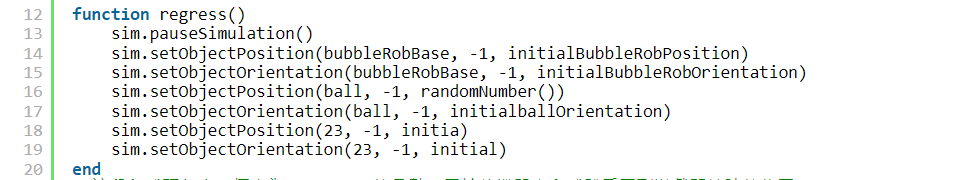
\includegraphics[width=12cm]{2}
\caption{\Large 改變顏色程式2}\label{改變顏色程式2}
\end{center}
\end{figure} 
\\
這段程式碼,如(圖.\ref{改變顏色程式2}),包含一個名為regress的函數,用於將機器人和球體重置到遊戲開始時的位置。在函數內部,程式暫停模擬運行,並使用sim.setObjectPosition 和sim.setObjectOrientation 函數將機器人和球體移回初始位置。\\
\newpage
\begin{figure}[hbt!]
\begin{center}
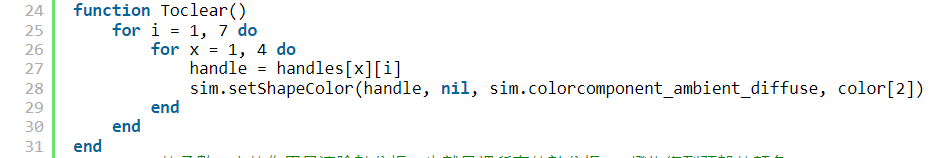
\includegraphics[width=12cm]{3}
\caption{\Large 改變顏色程式3}\label{改變顏色程式3}
\end{center}
\end{figure} 
如(圖.\ref{改變顏色程式3})Toclear的函數,它的作用是清除計分板,也就是把所有的計分板LED燈恢復到預設的顏色。函數使用了巢狀的for迴圈,首先從1到7執行一遍,然後再從1到4執行一遍,這樣就可以執行所有的計分板LED燈。在迴圈內部,函數通過handle變量獲取每個LED燈的控制句柄,然後使用sim.setShapeColor函數將其顏色設置為預設顏色 在color表中的索引為2的顏色。這樣,所有的計分板LED燈都會被恢復到預設的顏色,從而達到清除計分板的目的。\\
\\
\begin{figure}[hbt!]
\begin{center}
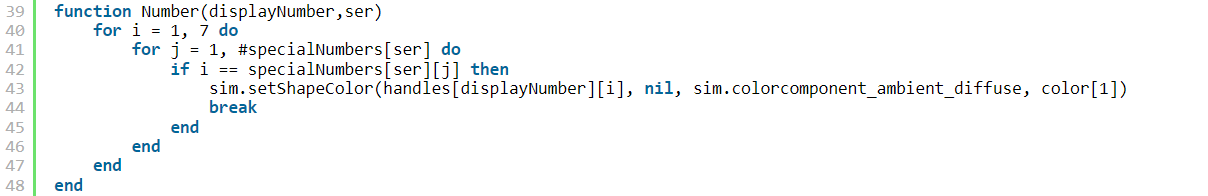
\includegraphics[width=12cm]{4}
\caption{\Large 改變顏色程式4}\label{改變顏色程式4}
\end{center}
\end{figure} 
這段程式碼,如(圖.\ref{改變顏色程式4})是一個顯示數字的函數,它有兩個參數,一個是要顯示的數字 displayNumber,另一個是顯示器的類型 ser。這個函數的作用是將 displayNumber 這個數字顯示在屏幕上,屏幕的類型由 ser 決定。 程式碼使用了嵌套的迴圈,第一個迴圈從 1 到 7 遍歷了七個數碼的 LED 顯示燈,第二個迴圈從 1 到 specialNumbers ser 的長度遍歷了指定類型的顯示屏上的特殊數碼。對於每個數碼燈,它會檢查這個燈是否是指定類型的顯示器的數字。如果是,它就會將該燈的顏色設置為顯示數字的顏色。\\
\newpage
\begin{figure}[hbt!]
\begin{center}
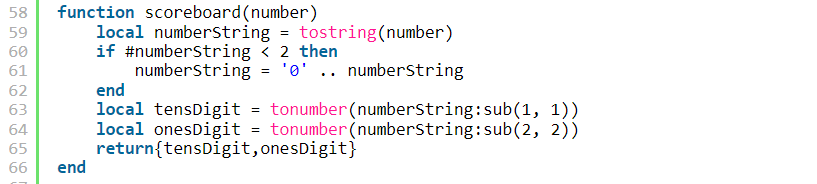
\includegraphics[width=12cm]{5}
\caption{\Large 改變顏色程式5}\label{改變顏色程式5}
\end{center}
\end{figure}\
如(圖.\ref{改變顏色程式5})這段程式碼定義了一個名為 scoreboard 的函數,該函數接受一個整數 number 作為參數,並將其轉換為兩位數的字串表示。如果傳入的 number 參數的長度小於2,則會在數字前面添加一個0,這樣就可以確保數字的表示總是兩位數。然後,這個函數會提取這個兩位數字串的每一位數字,分別存儲在一個名為 tensDigit 的變數和一個名為 onesDigit 的變數中。\
\begin{figure}[hbt!]
\begin{center}
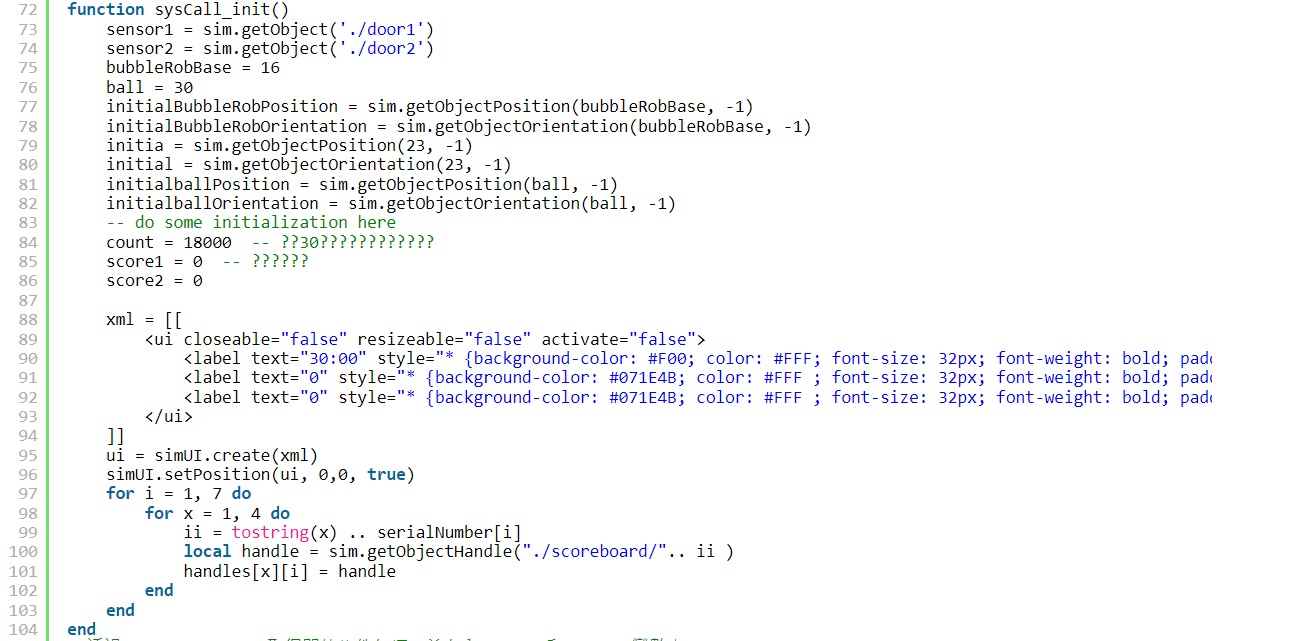
\includegraphics[width=12cm]{6}
\caption{\Large 改變顏色程式6}\label{改變顏色程式6}
\end{center}
\end{figure}\\
如(圖.\ref{改變顏色程式6}),透過sim.getObject 取得門的物件句柄,並存入sensor1和sensor2變數中。指定bubbleRobBase和ball變數分別為16和30,代表這些物件在模擬場景中的物件句柄。透過sim.getObjectPosition 和sim.getObjectOrientation 取得模擬場景中物件的位置和方向資訊,分別存入initialBubbleRobPosition、initialBubbleRobOrientation、initialballPosition和initialballOrientation變數中。將23號物件的位置和方向資訊分別存入initia和initial變數中。將count、score1和score2分別初始化為18000、0和0。創建一個簡單的UI介面,包含三個標籤label元件,分別代表倒數計時、兩個隊伍的得分。將介面移動到視窗左上角,並將其設為不可關閉、不可縮放和不可激活。設定用於記分牌的物件的物件句柄並存儲在handles二維陣列中。透過一個雙重迴圈,將所有的記分牌物件句柄存儲到handles變數中andles 是一個二維陣列,用於儲存多個物體在仿真環境中的句柄handle。二維陣列意味著它包含多個一維陣列,每個一維陣列都儲存了某一個維度上的物體句柄。在這裡,handles 有四個一維陣列,分別儲存了四個不同的元件在七個不同位置的句柄。通過這個二維陣列,程式可以方便地訪問並修改這些物體的屬性。\
\begin{figure}[hbt!]
\begin{center}
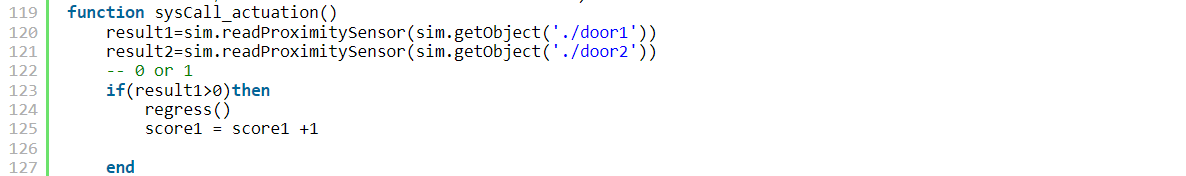
\includegraphics[width=12cm]{7}
\caption{\Large 改變顏色程式7}\label{改變顏色程式7}
\end{center}
\end{figure}\
\\
如(圖.\ref{改變顏色程式7}),此函數為一個回調函數,它會在仿真器每個時間步驟中被自動調用。在此函數中,首先透過sim.getObject 'door1' 和sim.getObject 'door2'獲取到與感測器關聯的對象。然後通過sim.readProximitySensor函數檢測與感測器對應的物體是否被觸發,並將檢測結果存儲在result1和result2變量中。如果result1大於0,表示感測器檢測到物體,此時會調用regress函數和加分操作,即分數score1加1。\
\begin{figure}[hbt!]
\begin{center}
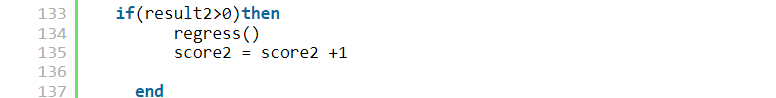
\includegraphics[width=12cm]{8}
\caption{\Large 改變顏色程式8}\label{改變顏色程式8}
\end{center}
\end{figure}\
\\
如(圖.\ref{改變顏色程式8}),如果result2大於0,表示感測器檢測到物體,此時會調用regress函數和加分操作,即分數score2加1。\
\newpage
\begin{figure}[hbt!]
\begin{center}
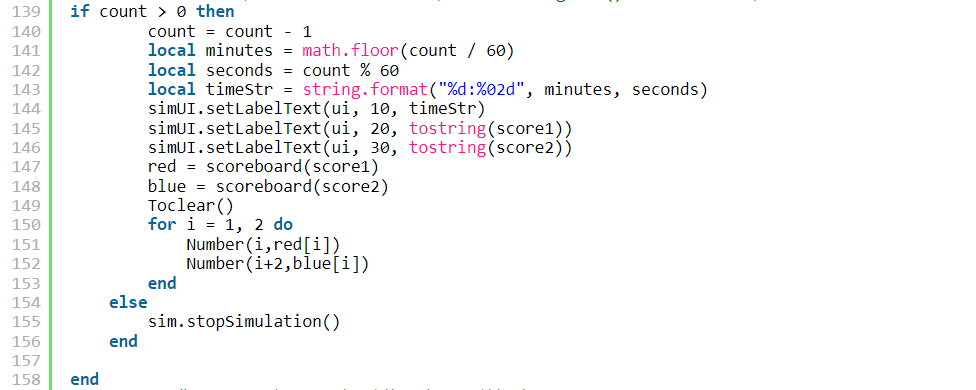
\includegraphics[width=12cm]{9}
\caption{\Large 改變顏色程式9}\label{改變顏色程式9}
\end{center}
\end{figure}\
如(圖.\ref{改變顏色程式9}),此段程式碼為在仿真環境中,用來更新計分板和倒數計時器的功能。當遊戲倒數計時器仍有剩餘時間count 大於 0,會依照每個計數間隔1秒進行更新。更新內容包含:剩餘時間的計算、將計算後的時間顯示在UI的倒數計時器上、顯示當前紅藍雙方的得分,同樣也是透過UI的label顯示。接著,程式會進入計分板的顯示功能。這邊透過呼叫Toclear,先清除所有計分板的數字。再透過迴圈讀取紅藍雙方的分數,分別呼叫Number函數,在計分板上顯示對應的數字。若遊戲倒數計時器已歸零,則程式會執行sim.stopSimulation,停止遊戲仿真。\
\begin{figure}[hbt!]
\begin{center}
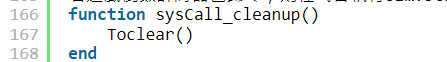
\includegraphics[width=12cm]{10}
\caption{\Large 改變顏色程式10}\label{改變顏色程式10}
\end{center}
\end{figure}\
如(圖.\ref{改變顏色程式10}),此程式為清理函數,當仿真停止時,會呼叫此函數,其目的為將目前顯示在分數板上的數字全部清除,使得下一次的遊戲能夠從零開始顯示分數。在此函數中,會呼叫之前已定義的Toclear函數,該函數會將所有的數字方塊改變為背景色,以達到清空的效果。\
\newpage
\section{機械式程式講解}
\begin{figure}[hbt!]
\begin{center}
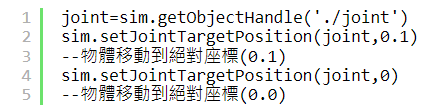
\includegraphics[width=12cm]{1-1}
\caption{\Large 機械式程式}\label{機械式程式}
\end{center}
\end{figure}\
如(圖.\ref{機械式程式}),完成馬達操控。\\
\
\begin{figure}[hbt!]
\begin{center}
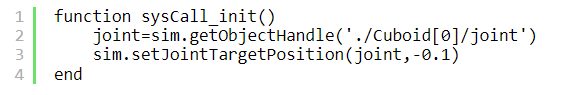
\includegraphics[width=12cm]{1-2}
\caption{\Large 機械式程式2}\label{機械式程式2}
\end{center}
\end{figure}\\
\
如(圖.\ref{機械式程式2}),測試記分板顯示數字0。\